\subsection{Diagramas de Secuencia}
\label{subsec:diagramas_secuencia_quejoso}

Los diagramas de secuencia presentados en esta sección modelan la interacción cronológica entre los objetos del sistema para ejecutar las funciones más críticas del módulo del quejoso. 
El diseño respeta una arquitectura de tres capas donde la Capa de Presentación (Angular) interactúa con la Capa de Negocio (Spring Boot Services) a través de controladores REST, y esta última gestiona la persistencia mediante la Capa de Datos (PostgreSQL). Se ha priorizado el modelado del camino esperado y las validaciones de seguridad fundamentales, como la encriptación de contraseñas y la generación de folios únicos.

\subsubsection{CU01: Levantar una queja}
Este diagrama ilustra el proceso de registro inicial de una vulneración de derechos. Describe el flujo de la queja para llegar a la generación automática de un folio digital único y el cambio de estatus de la entidad a "RECIBIDA" antes de su persistencia en la base de datos.

\begin{figure}[H]
    \centering
    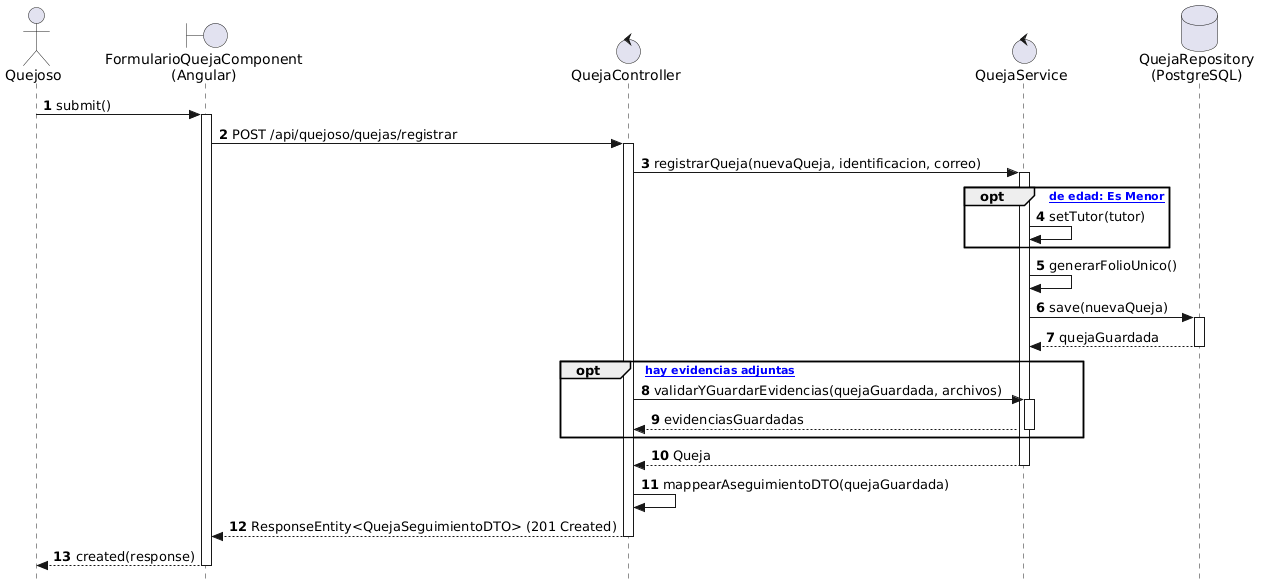
\includegraphics[width=\textwidth]{imagenes/quejoso/D_Secuencia/DS01-LevantarQueja.png}
    \caption{Diagrama de Secuencia: CU01 Levantar Queja}
    \label{fig:ds01_levantar_queja}
\end{figure}

\subsubsection{CU03: Crear Cuenta (Activación con Folio)}
Representa la transición de un usuario invitado a uno autenticado. El flujo muestra la validación cruzada entre el nuevo registro de usuario y la existencia previa de un folio de queja, asegurando que la cuenta quede vinculada correctamente al historial del solicitante.

\begin{figure}[H]
    \centering
    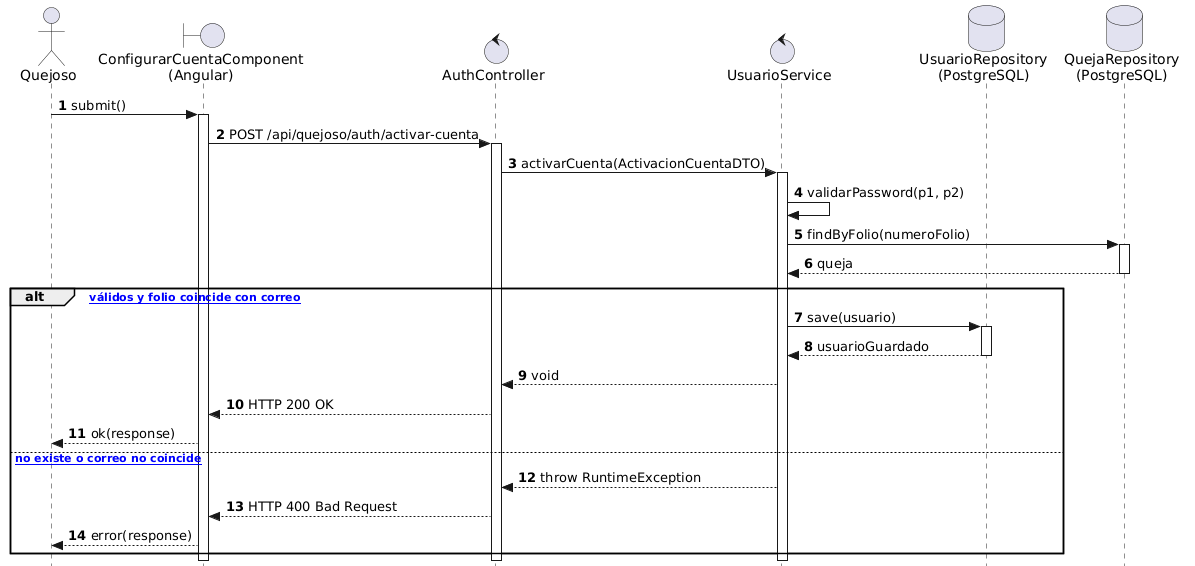
\includegraphics[width=\textwidth]{imagenes/quejoso/D_Secuencia/DS02-CrearCuenta.png}
    \caption{Diagrama de Secuencia: CU03 Crear Cuenta (Activación)}
    \label{fig:ds02_crear_cuenta}
\end{figure}

\subsubsection{CU04: Descargar Acuse}
Documenta la generación dinámica de documentos oficiales en formato PDF. El diagrama muestra cómo el sistema recupera los datos del expediente desde la base de datos para alimentar el motor de plantillas y transmitir el archivo final al navegador del usuario.

\begin{figure}[H]
    \centering
    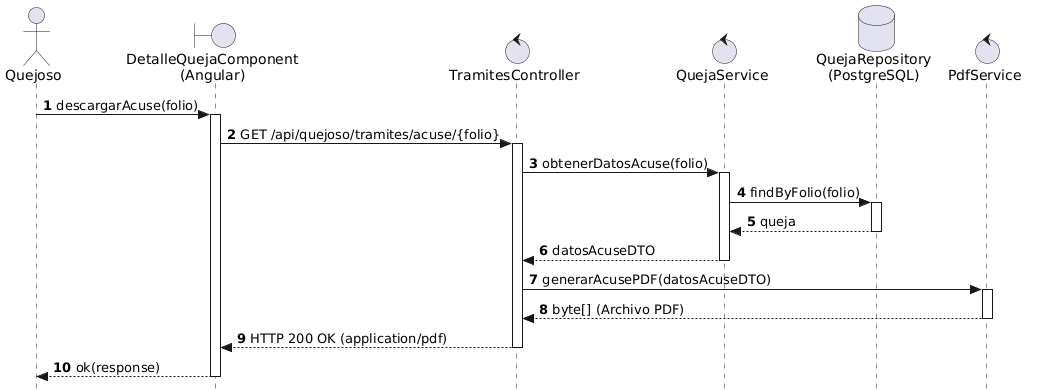
\includegraphics[width=\textwidth]{imagenes/quejoso/D_Secuencia/DS03-DescargarAcuse.png}
    \caption{Diagrama de Secuencia: CU04 Descargar Acuses}
    \label{fig:ds03_descargar_acuse}
\end{figure}

\subsubsection{CU06: Iniciar Sesión}
Este diagrama detalla el protocolo de seguridad para el acceso al Dashboard. Se enfatiza el uso del componente PasswordEncoder para la validación criptográfica de credenciales y la generación de un token JWT para mantener la sesión activa de forma segura.

\begin{figure}[H]
    \centering
    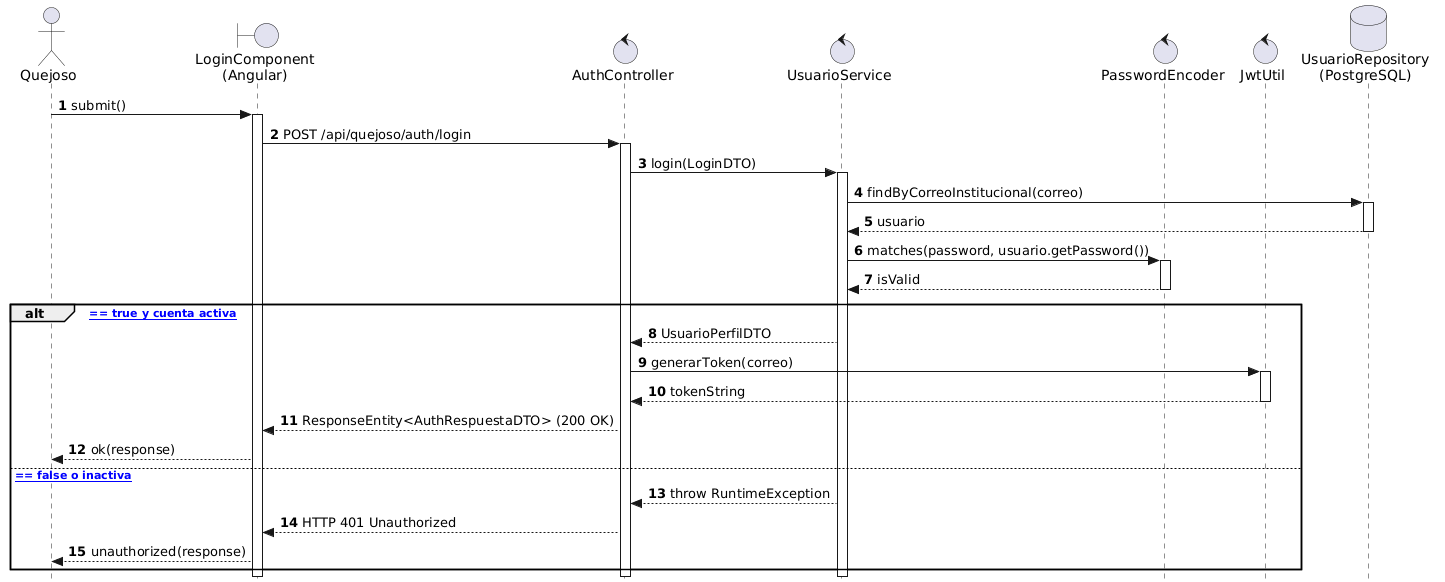
\includegraphics[width=\textwidth]{imagenes/quejoso/D_Secuencia/DS04-Login.png}
    \caption{Diagrama de Secuencia: CU06 Iniciar Sesión}
    \label{fig:ds04_login}
\end{figure}

\subsubsection{CU07: Recuperar Contraseña}
Describe el proceso de restablecimiento de acceso mediante el envío de un código de seguridad por correo electrónico (protocolo SMTP). Incluye la validación de identidad y la actualización segura (encriptada) de la nueva contraseña en la base de datos.

\begin{figure}[H]
    \centering
    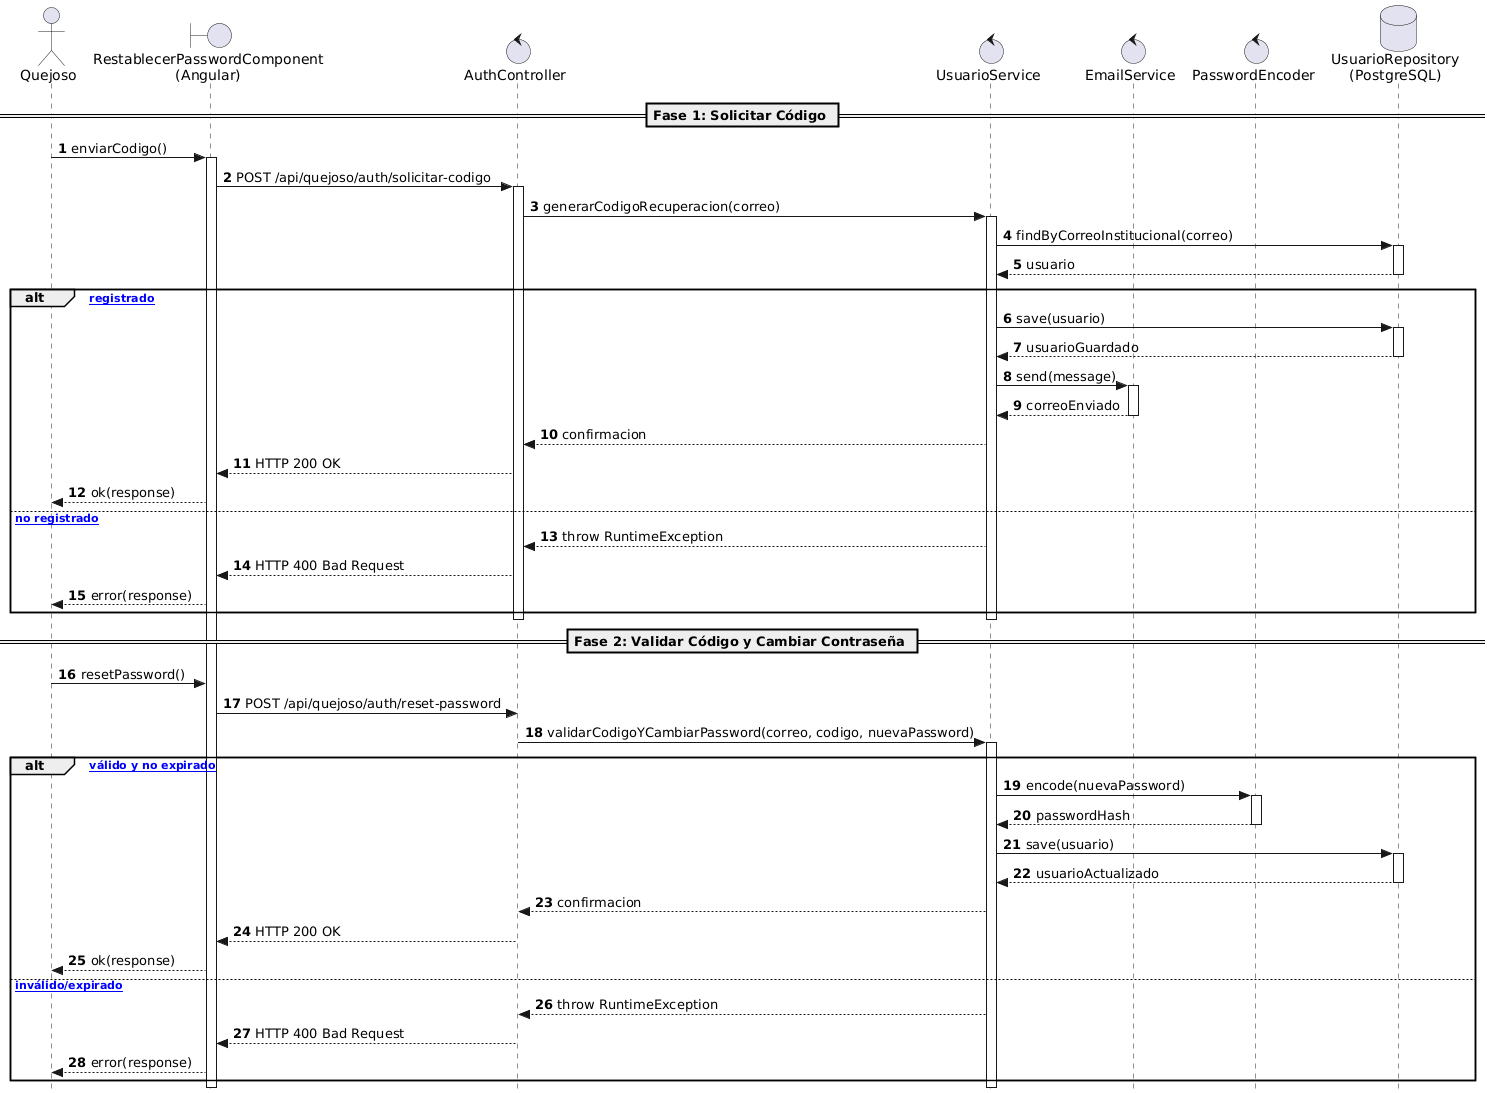
\includegraphics[width=\textwidth]{imagenes/quejoso/D_Secuencia/DS05-RecupPass.png}
    \caption{Diagrama de Secuencia: CU07 Recuperar Contraseña}
    \label{fig:ds05_recup_pass}
\end{figure}

\subsubsection{CU09: Modificar queja}
Este diagrama detalla el proceso mediante el cual un quejoso puede actualizar la información de un expediente que aún se encuentra en estatus "RECIBIDA".
Este diagrama representa la secuencia completa de la modificación de una queja. Se destaca el uso de un fragmento de referencia (ref) que invoca la lógica de gestión de archivos. El flujo modela cómo el servicio de Spring Boot recupera la entidad existente, aplica los cambios en la narrativa y procesa atómicamente la eliminación o adición de evidencias antes de persistir los cambios finales en la base de datos.

\begin{figure}[H]
    \centering
    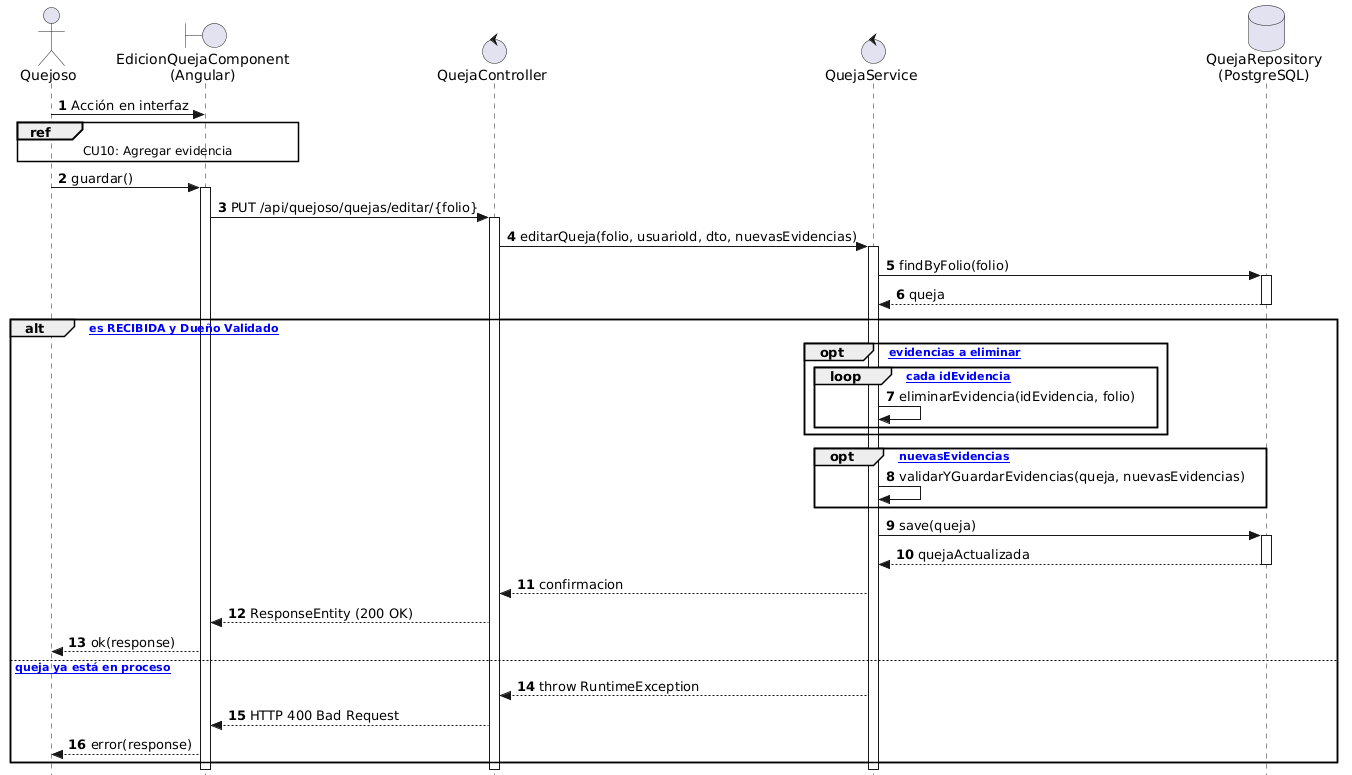
\includegraphics[width=\textwidth]{imagenes/quejoso/D_Secuencia/DS06-ModificarQueja.png}
    \caption{Diagrama de Secuencia: CU09 Modificar Queja}
    \label{fig:ds06_modificar_queja}
\end{figure}

\subsubsection{CU10: Agregar evidencia}
Este diagrama modela la funcionalidad de adjuntar archivos adicionales a una queja existente. Se muestra cómo el sistema maneja la carga de archivos, su almacenamiento seguro (posiblemente en un servicio de almacenamiento externo) y la actualización de la entidad de queja para incluir referencias a las nuevas evidencias, asegurando la integridad y trazabilidad de los datos.

\begin{figure}[H]
    \centering
    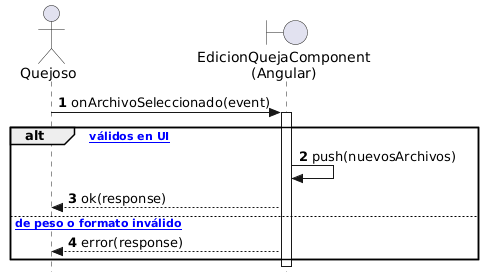
\includegraphics[width=\textwidth]{imagenes/quejoso/D_Secuencia/DS07-AdjuntarEvidencia.png}
    \caption{Diagrama de Secuencia: CU10 Agregar Evidencia}
    \label{fig:ds07_adjuntar_evidencia}
\end{figure}

\subsubsection{CU17: Aceptar/Rechazar Propuesta de Conciliación}
Modela una transacción de negocio decisiva donde el quejoso ejerce su derecho de respuesta ante una propuesta de la Defensoría. El flujo garantiza que el cambio de estatus del expediente sea irreversible y quede debidamente justificado en caso de rechazo.

\begin{figure}[H]
    \centering
    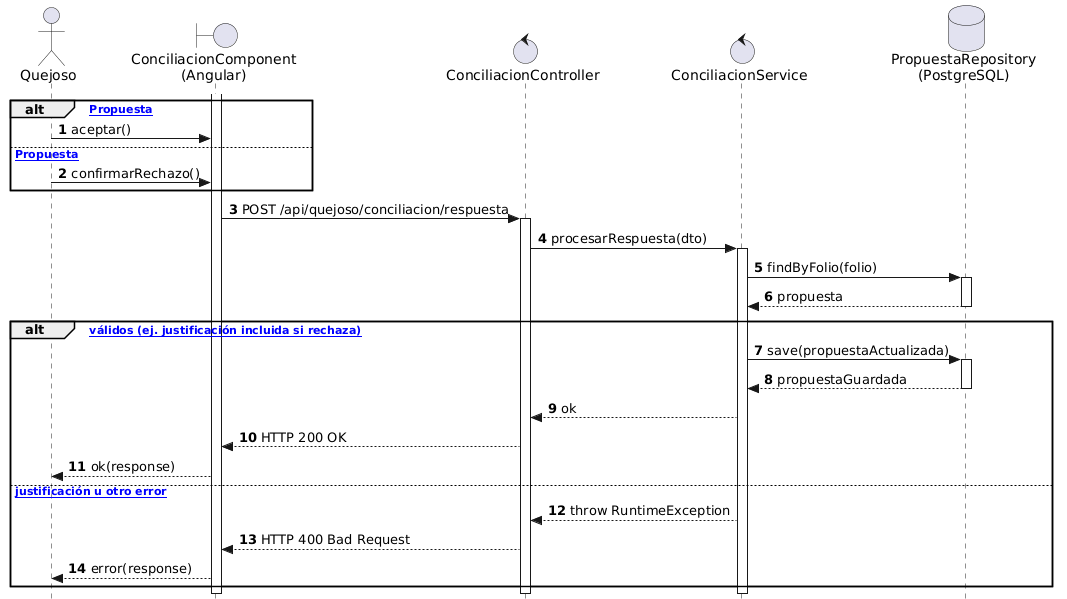
\includegraphics[width=\textwidth]{imagenes/quejoso/D_Secuencia/DS08-PropuestasConciliacion.png}
    \caption{Diagrama de Secuencia: CU17 Aceptar/Rechazar Propuesta de Conciliación}
    \label{fig:ds08_propuestas_conciliacion}
\end{figure}

\subsubsection{CU20: Actualizar Datos de Contacto y/o Tutor}
Ilustra el mantenimiento de la información de perfil. El diagrama modela el proceso completo de recuperación de datos existentes, validación de nuevos formatos y persistencia de cambios para asegurar canales de comunicación vigentes.

\begin{figure}[H]
    \centering
    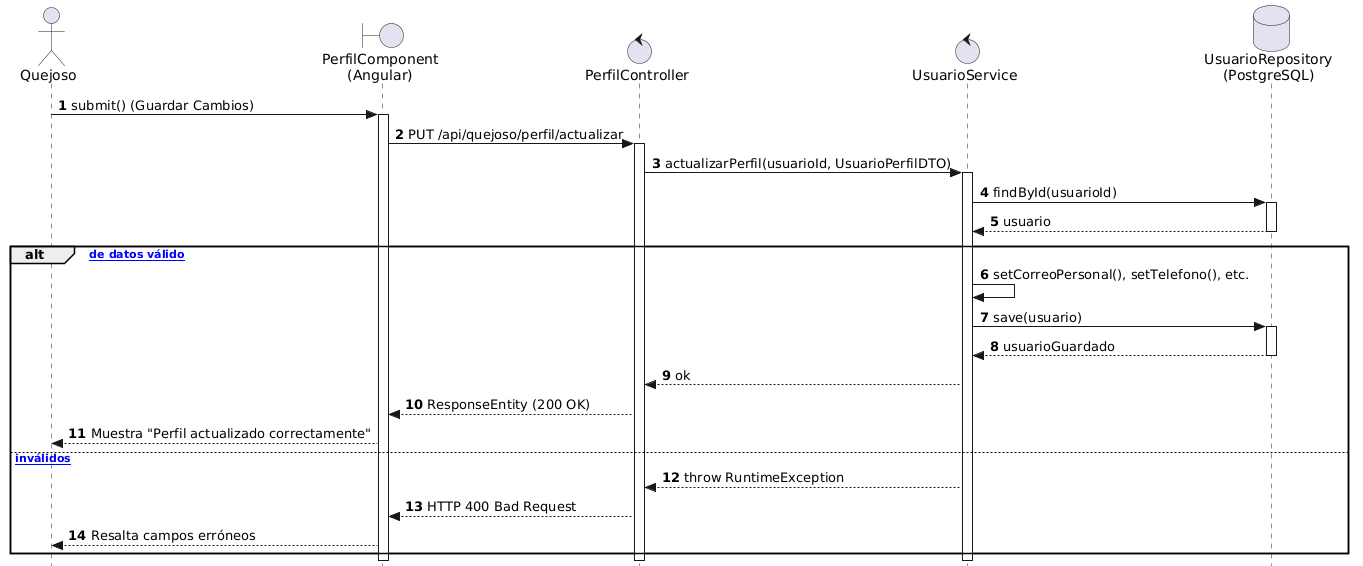
\includegraphics[width=\textwidth]{imagenes/quejoso/D_Secuencia/DS09-ActDatosContacto.png}
    \caption{Diagrama de Secuencia: CU20 Actualizar Datos de Contacto y/o Tutor}
    \label{fig:ds09_act_datos_contacto}
\end{figure}
